\chapter{Progettazione logica della soluzione proposta}
\label{chap:Prog_log_sol}

Il nostro studio era mirato alla ricerca un possibile modo di diffondere messaggi e informazioni tra la popolazione, in situazioni dove le principali reti di comunicazione non sono disponibili. Ci siamo quindi concentrati su ciò che rimane disponibile in questi scenari e quali siano i metodi per modellare la situazione. Ci siamo concentrati sullo sfruttare ciò che è di più comune uso, ciò che è molto diffuso e facilmente in possesso di ogni persona. Da questo studio è risultato che gli smartphone rispecchiano questo profilo, infatti, al giorno d'oggi in media ogni persona possiede uno smartphone. Siamo passati quindi a studiare ciò che uno smartphone potesse fornire o ciò che di utile avremmo potuto sfruttare. Uno smartphone, ma in generale ogni dispositivo mobile, senza la presenza delle comuni reti di comunicazione, quali internet e telefonia, ha solo altri due modi di poter comunicare con altri dispositivi mobili: la tecnologia a infrarossi e la tecnologia Bluetooth. Da un rapido studio è emerso che la scelta degli infrarossi non avrebbe avuto portato a una soluzione performante e applicabile, mentre il Bluetooth si è rivelato essere un ottimo punto di partenza per un caso di studio. Il sistema Bluetooth in generale, come presentato nella \MySec{sec:ble}, è un sistema di comunicazione Peer-to-Peer e quindi permetterebbe di mettere in comunicazione due dispositivi mobili anche in assenza delle reti di comunicazione. A questo punto ci siamo concentrati sul capire come poter sfruttare questa tecnologia per progettare una soluzione. Gli aspetti principali studiati sono: il modello di rete da utilizzare, il metodo con cui guidare e gestire la diffusione dell'informazione e infine come tutto ciò vada a impattare sul consumo energetico dei dispositivi. Un altro aspetto fondamentale di questo lavoro è stato tenere in considerazione il consumo energetico aggiuntivo che si va a introdurre su singolo dispositivo, poiché se l'impatto energetico fosse troppo elevato, si avrebbe una considerevole riduzione nell'autonomia del dispositivo stesso, rendendo la soluzione proposta impraticabile.

Abbiamo fatto, come prima cosa, uno studio sul consumo energetico richiesto da una singola trasmissione dati tramite \acs{BLE}. Abbiamo poi studiato diversi casi, in cui abbiamo fatto variare la grandezza del pacchetto trasmesso e valutato i consumi energetici richiesti. Dal nostro studio è emerso che l'energia richiesta per il trasferimento di una singola informazione, anche di discrete dimensioni, non vada a inficiare in maniera gravosa il consumo energetico medio dei più comuni smartphone in commercio.  Lo standard \acs{BLE} utilizza molti parametri per qualsiasi evento di trasmissione o ricezione. Abbiamo utilizzato Excel per costruire un modello in grado di simulare calcolare il tempo impiegato per la trasmissione di un'informazione, specificandone la grandezza e tutti i parametri che caratterizzano la trasmissione \acs{BLE}. Molti parametri possono variare su intervalli piuttosto larghi, ma come illustrato nella documentazione ufficiale \cite{BT-CoreSpec4.0} e anche in \cite{sensor2012}, più i valori dei parametri crescono più il consumo energetico richiesto mediamente diminuisce. Questo perché aumentano i tempi di riposo e diminuiscono i momenti in cui il dispositivo deve rendersi attivo per trasmettere o ricevere; ovviamente questo va a discapito delle prestazioni in termini di ritardi. Per questo motivo, nel nostro studio abbiamo mantenuto tutti i parametri ai loro valori minimi per studiare il caso di massimo consumo energetico medio e anche di massima prestazione.

Nel nostro studio abbiamo fatto variare la grandezza dell'informazione da pochi Byte fino a 200 MB, in modo da vedere il comportamento con informazioni grandi e realmente possibili. In \myFig{fig:cons_en_sing_tx} riportiamo su grafico i risultati ottenuti e, come si può notare, dopo un certo valore, l'andamento del consumo energetico rimane lineare e diretto con la grandezza dell'informazione. L'andamento iniziale molto basso è dovuto alla predominazione dei tempi di attesa e connessione dello standard BLE sul tempo di trasmissione dell'informazione. La trasmissione dati su BLE prevede che dopo un'attesa variabile iniziale, la trasmissione avvenga tramite connection event consecutivi; un connection event è un evento nel quale sono scambiati dati tra due dispositivi connessi tra loro. Infine abbiamo stimato quante trasmissioni un dispositivo possa affrontare, oltre al suo carico medio di lavoro prima di scaricarsi. Il calcolo prevede che si parta sempre a batteria completamente carica e abbiamo considerato i più comuni e attuali smartphone sul mercato. La stima ovviamente dipende dalla grandezza dell'informazione e varia da un minimo attorno alle 200 trasmissioni fino a un massimo nell'intorno delle 400 trasmissioni.

\begin{figure}[tbh]
	\centering
	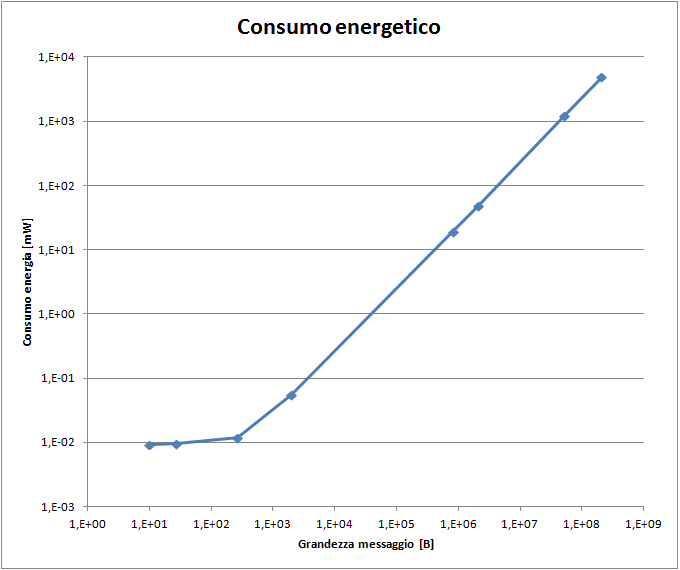
\includegraphics[width=0.7\linewidth]{Images/studio_energetico/cons_en_sing_tx}
	\caption[Studio energetico]{Energia media richiesta per il trasferimento di una informazione.}
	\label{fig:cons_en_sing_tx}
\end{figure}
\bigskip

Lo studio sul consumo energetico ci ha confermato che il basso livello di energia richiesto dalla tecnologia BLE per la trasmissione di informazioni, anche di medie dimensioni, permette di sfruttare questo sistema di comunicazione per diffondere messaggi tra nodi mobili. Dato il poco consumo energetico, la nostra soluzione prevede che il dispositivo mobile non debba dedicarsi completamente a questo servizio, anzi esso rimarrà sempre a disposizione dell'utente senza che il nostro sistema limiti all'utente l'uso del dispositivo. Questo perché ormai sui dispositivi mobile, quali smartphone o tablet ad esempio, vi sono tante altre applicazioni o funzioni utili all'utente che debbano rimanere fruibili in ogni situazione, anche in scenari come quelli da noi ipotizzati.

Dopo l'aspetto energetico, ci siamo dedicati allo studio di un modello di rete che potesse descrivere correttamente la disposizione dei dispositivi e del mezzo di comunicazione. Il BLE, ma la tecnologia Bluetooth in generale, è un sistema di comunicazione molto legato alla potenza del trasmettitore e dalla relativa distanza che tale potenza consente di raggiungere. Per questo motivo abbiamo scelto di modellare la nostra rete di dispositivi mobili con una Random Geometric Graph, presentata nella \MySec{subsec:modelli_rete}. La scelta di questo modello di rete è stata abbastanza naturale, visto la comune caratteristica che caratterizza la trasmissione \acs{BT} e il modello di rete stesso.

Infine dopo l'aspetto del modello di rete, ci siamo dedicati allo studio di un sistema di regole che potessero governare la diffusione delle informazioni. Dopo un'attenta analisi è emerso che per com'è composta la rete e per il tipo d'informazioni, un modo efficace di diffondere informazioni è quello del passa parola. Per questo motivo abbiamo preso in considerazione il mondo degli algoritmi di gossip, o epidemici, creati per modellare la diffusione d'informazioni tra le persone e sui social network, o nel caso degli epidemici come si diffonde un'epidemia in una popolazione. Tra gli algoritmi di gossip, abbiamo scelto di estendere l'algoritmo del \acl{FF}, un algoritmo di gossip di tipo Rumor Mongering presentato nella \MySec{subsec:alg_p2p}. La nostra soluzione è stata progettata perché tenga in considerazione il consumo energetico che essa genera sul dispositivo. Per questo motivo abbiamo progettato il nostro algoritmo, estendendo quello già esistente, aggiungendo elementi molto dinamici. Infatti, i parametri da noi progettati, regolano l'algoritmo in modo dinamico, permettendogli di adattarsi allo stato dell'ambiente esterno e allo stato interno del dispositivo. Per stato dell'ambiente esterno intendiamo il numero di dispositivi presenti nelle vicinanze, quindi lo stato della rete attorno al dispositivo, mentre per stato interno intendiamo il livello della batteria, in modo da regolare lo “sforzo” in maniera corretta. Il nostro algoritmo cerca sempre di regolare i parametri in modo da garantire un buon compromesso tra prestazioni e consumo energetico/carico di lavoro. Dopo un'attenta analisi abbiamo deciso di progettare l'algoritmo con due differenti valori di reattività, di fronte a cambiamenti nella rete o nello stato interno del dispositivo oppure in entrambi.
\bigskip

\section{Modello di rete}
Dopo aver ricercato in letteratura, abbiamo capito che il modello di rete di tipo Peer-to-Peer è adatto a modellare la rete che abbiamo studiato. Le \acs{P2P} sono reti di nodi totalmente paritetici, senza alcuna struttura gerarchica o differenziazione tra i nodi stessi. Per questo motivo ogni nodo della rete è chiamato peer e lo scambio d'informazioni avviene sempre tra due peer alla volta. Tra i tanti modelli presenti in letteratura, abbiamo scelto quello che riesce a rappresentare al meglio le caratteristiche della rete da noi in esame: il modello che abbiamo scelto è il \acf{RGG}. Questo tipo di modello è costituito da un grafo \textit{G(N,$\rho$)} bidirezionale casuale inserito in un'area limitata ed è composto da N nodi. Il parametro $\rho$ rappresenta la distanza massima entro la quale sono stabiliti i collegamenti tra i nodi. Il raggio $\rho$ è di fatto la distanza geometrica entro la quale un nodo stabilisce collegamenti con altri nodi. Due nodi a una distanza inferiore di $\rho$ avranno un collegamento bidirezionale, mentre due nodi a una distanza maggiore di $\rho$ non avranno nessun collegamento tra loro. Questo tipo di modello presenta una basa degree variance, ma un'alta edge dependency. Sono due parametri che rispettivamente indicano la varianza nella distribuzione del grado dei nodi e un fattore di dipendenza dagli archi del grafo che indica la probabilità che vi siano collegamenti tra nodi vicini.

Nel nostro caso di studio il raggio $\rho$ modella la portata del trasmettitore Bluetooth, infatti, solo dispositivi che si trovano entro il raggio d'azione dei rispettivi trasmettitori possono comunicare, mentre dispositivi fuori portata non avranno alcun collegamento. La costruzione di un \acs{RGG} inizia scegliendo le caratteristiche dell'area, base e altezza. Successivamente si dispongono in maniera casuale uniforme i nodi del grafo all'interno dell'area. Infine si controllano le distanze tra tutti i nodi e si instaurano i collegamenti solo trai i nodi a una distanza uguale o inferiore a $\rho$. In figura \ref{alg:gossipFFrgg_gen} sono riportati due esempi di \acs{RGG}.

\begin{figure}[t]
	\subfloat[\label{subfig-1:rgg_03}]{%
		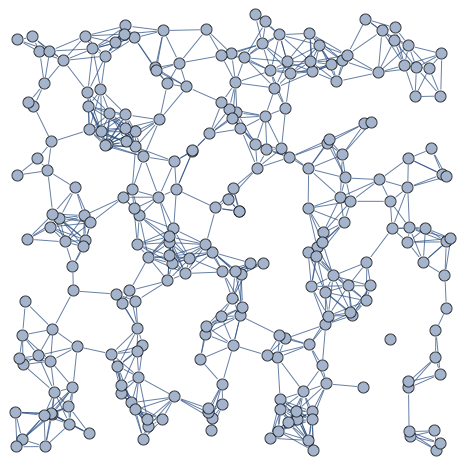
\includegraphics[width=0.45\textwidth, keepaspectratio]{Images/reti/RandomGeometricGraph_03}
	}
	\hfill
	\subfloat[\label{subfig-2:rgg_06}]{%
		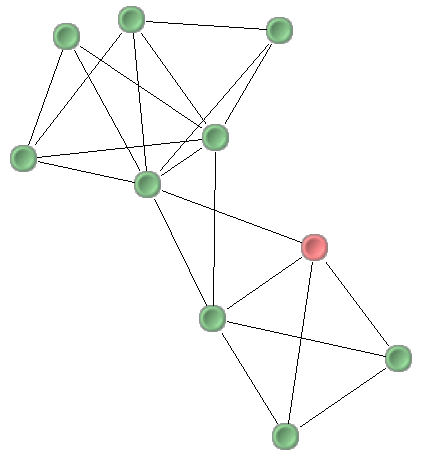
\includegraphics[width=0.45\textwidth, keepaspectratio]{Images/reti/RandomGeometricGraph_06}
	}
	\caption{Esempio di file di inizializzazione.}
	\label{fig:rgg_gen}
\end{figure}

Com'è possibile intuire, il parametro $\rho$ è la chiave principale che determina quanto sia connesso il grafo. Più $\rho$ è piccolo più la probabilità di avere sottografi isolati e/o archi \textit{bridge} tra i sottografi è elevata. Un bridge è un arco singolo che collega un nodo di un sottografo con un nodo di un altro sottografo, rendendo quell'arco l'unica possibile via di comunicazione tra i due sottografi. Un raggio ridotto, diminuisce la possibilità di avere collegamenti ridondanti per la diffusione dell'informazione e aumenta la possibilità di avere gruppi di nodi isolati e la formazione di bottleneck nella rete. Al contrario, più il raggio cresce più la probabilità di avere nodi o sottogruppi di nodi isolati diminuisce, come anche la probabilità di avere archi bottleneck e la rete tenderà a essere sempre più connessa. Va detto anche che oltre al raggio $\rho$, è altrettanto importante la dimensione dell'area in cui la rete si trova. Nonostante l'area non sia un parametro del grafo, essa influisce, insieme a $\rho$, a rendere il grafo più o meno connesso. Il motivo è dovuto al metodo con cui è generato il grafo. Presa un'area, i nodi vengono distribuiti in modo casuale e uniforme all'interno dell'area. Più l'area è grande, più la distribuzione uniforme tenderà a disperdere i nodi. Dato un grafo con N e $\rho$ fissati, più l'area è grande più la densità dei nodi per metro quadro sarà bassa, mentre al contrario, più l'area è piccola più la densità sarà elevata. Questo fattore di dispersione ci ha permesso di poter simulare scenari diversi, dal grosso centro urbano con alta densità abitativa, fino al paese di campagna dove la popolazione è molto più diradata. Per questo motivo, è stato importante lavorare secondo ipotesi di diverse densità di nodi; fissati densità e numero di nodi, l'area è calcolata di conseguenza. Come già detto in precedenza, il nostro algoritmo presenta una componente dinamica, che tiene in considerazione le variazioni dell'ambiente esterno. Negli scenari da noi considerati, è molto facile che la densità di popolazione possa variare e per questo motivo abbiamo implementato moduli specifici che hanno lo scopo di seguire questi cambiamenti.

\section{Sistema di trasmissione}
Abbiamo scelto di utilizzare il Bluetooth Low Energy come mezzo di comunicazione perché, in situazioni di assenza di tutte le altre reti di comunicazione, esso rimane comunque operativo. Il BLE, presentato nella \MySec{sec:ble}, è uno standard di comunicazione Peer-To-Peer ufficializzato nel 2010. Nella sua versione 4.0, la casa produttrice ha presentato uno standard denominato Low Energy, infatti, questa nuova tecnologia ha consumi ridotti anche di dieci volte rispetto alle sue versioni precedenti. Ciò ha contribuito alla sempre maggior diffusione e utilizzo di questo standard nei settori del monitoraggio ambientale, della sensoristica, dei dispositivi wearable in coppia con i dispositivi mobile. Questa tecnologia è stata sviluppata per lo scambio di piccoli dati tra due enti e quindi ottimizzando i consumi energetici per questo tipo di carico di lavoro; il BLE non è stato progettato per lo streaming. Questo standard presenta ridotti tempi di latenza e parametri di connessione più semplici, rendendo più veloce connettersi a un dispositivo. Questo standard è equipaggiato su ogni dispositivo mobile in commercio e i modelli più recenti sono già dotati della versione 4.1. Da un indagine ISTAT \cite{istat2014} del 18 Dicembre 2014, le percentuali sulla presenza della tecnologia all'interno delle famiglie italiane sono tutte in crescita, come la presenza di una connessione a Internet salita 64\% o di una connessione a banda larga salita a quasi il 63\%, ma dato più significativo per noi è stato quello dei telefoni cellulari, che sono presenti in più del 93\% delle famiglie italiane. L'uso di Internet tramite smartphone è cresciuto dal 20.8\% al 28\% e ciò sta a indicare un rinnovamento anche nei dispositivi stessi; le persone acquistano dispositivi più recenti che permettano loro di navigare più facilmente su Internet. Sempre dall'analisi ISTAT è emerso che il 22.4\% delle persone che navigano su Internet dai 14 anni in su lo ha fatto tramite un computer, mentre il 35.4\% degli utenti tramite cellulare o smartphone e solo il 6\% da altri dispositivi mobili. L'utilizzo dello smartphone è la tipologia di dispositivi più utilizzata per l'accesso a Internet. Per questo motivo abbiamo formulato l'ipotesi che ogni persona possieda uno smartphone e che possa essere rappresentata da esso nella nostra rete. Per questi motivi abbiamo scelto come strumento di comunicazione la tecnologia \acs{BLE}.

Richiamiamo brevemente la macchina a stati che rappresenta il funzionamento del Link Layer del \acs{BLE}. Essa è composta dai seguenti cinque stati:
\begin{itemize}
	\item \textbf{Standby}: stato raggiungibile da tutti gli altri stati. In questo stato non è possibile effettuare nessuna trasmissione di pacchetti né riceverne.
	\item \textbf{Advertising}: un dispositivo in questo stato si chiama advertiser e può inviare pacchetti di advertiser. Resta in ascolto per pacchetti in risposta ai suoi pacchetti di advertisinge.
	\item \textbf{Scanning}: un dispositivo in questo stato si chiama scannar e ricompre il ruolo di osservatore. Rimane in ascolto per pacchetti di advertising.
	\item \textbf{Initiating}: stato raggiungibile da tutti gli altri stati. In questo stato non è possibile effettuare nessuna trasmissione di pacchetti né riceverne.
	\item \textbf{Standby}: un dispositivo in questo stato si chiama initiator e rimane in ascolto di pacchetti di advertising. Risponderà a quei pacchetti di advertising ai quali è interessato, con un pacchetto di \textit{connection request} con l'intenzione di aprire una connessione.
	\item \textbf{Connection}: lo stato di Connection può essere raggiunto sia dallo stato di Advertising sia dallo stato di Initiating. Indica che il dispositivo sta tentando di connettersi o è connesso con un altro dispositivo. Lo stato Connection si suddivide in due ruoli: Slave e Master.
	\begin{itemize}
		\item \textbf{Slave}: il ruolo di Slave è affidato a chi arriva nello stato di Connection dallo stato di Advertising. Utilizza i parametri di connessione decisi/inviategli dal Master.
		\item \textbf{Master}: il ruolo di Master è affidato a chi arriva nello stato di Connection dallo stato di Initiator. Un dispositivo Master decide i parametri della connessione, che invierà allo Slave.
	\end{itemize}
\end{itemize}
Nell'implementazione della nostra soluzione abbiamo mappato uno a uno gli stati del BLE con gli stati dell'algoritmo di gossip scelto, che descriveremo nella sezione successiva, in modo da avere una corrispondenza tra stato di trasmissione con stato di contagio.
In \myFig{fig:bt_fsa2} richiamiamo la macchina a stati del BLE.
\begin{figure}[tb]
	\centering
	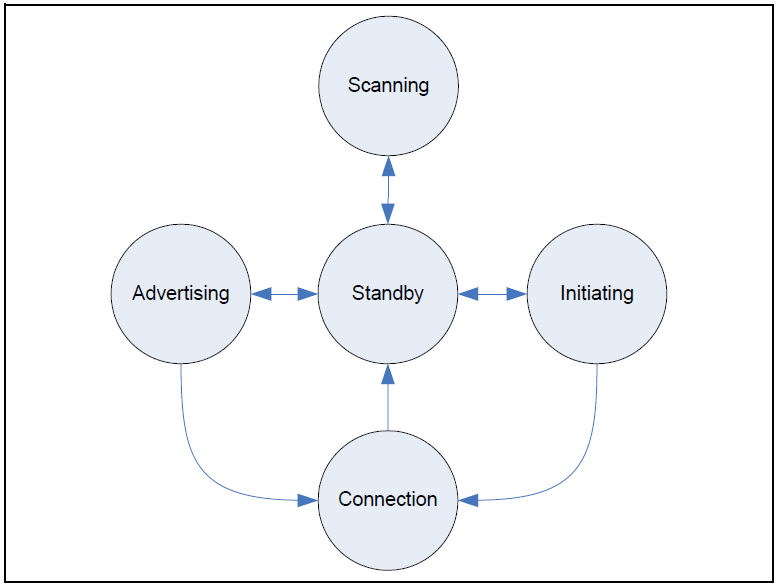
\includegraphics[width=0.7\linewidth]{Images/bt/bt_fsa}
	\caption[ble fsa]{Macchina a stati del Link Layer del BLE.}
	\label{fig:bt_fsa2}
\end{figure}
\bigskip

\section{Soluzione: Algoritmo Dynamic Fanout}
Dopo una profonda analisi degli algoritmi di gossip presenti in letteratura e della loro classificazione, abbiamo deciso di basare la nostra soluzione su algoritmi di tipo Rumor Mongering, in altre parole algoritmi che hanno come obiettivo la diffusione di un “rumore” o pettegolezzo, nel nostro caso un'informazione. Nella \MySec{subsec:alg_p2p} abbiamo presentato alcuni algoritmi di gossip adatti a reti \acs{P2P} e i diversi aspetti che li caratterizzano. La nostra scelta è stata di usare come base l'algoritmo del Fixed Fanout, per poi estenderlo con l'aggiunta di parametri dinamici, allo scopo di dare appunto dinamicità all'algoritmo e capacità di adattamento ai diversi cambiamenti dell'ambiente esterno e dello stato interno dei dispositivi stessi. Con cambiamenti dell'ambiente estero intendiamo le variazioni della rete nel raggio d'azione del nodo, quindi il variare del numero di nodi che esso percepisce, mentre con variazioni interne al dispositivo intendiamo la carica/scarica della batteria. Questo perché abbiamo cercato di progettare i parametri in modo che abbiano sempre un valore che possa garantire prestazioni accettabili e che calibri il carico di lavoro del dispositivo in relazione al livello energetico che la batteria ha. Se il livello di energia è elevato, l'algoritmo cerca di assegnare al dispositivo un carico di lavoro maggiore se necessario, mentre se il livello di energia è medio basso, l'algoritmo comincia a calibrare i parametri in modo da trovare un compromesso di carico di lavoro ed efficienza in modo da non gravare molto sulla restante poca autonomia del dispositivo. Dato che il sistema non è né un sistema dedicato né occupa completamente le risorse di calcolo del dispositivo, non vogliamo privare l'utente degli eventuali altri servizi presenti sul suo smartphone che possano servirgli. Per questo motivo l'algoritmo, dopo che la batteria scende sotto una certa soglia limite, pone il sistema in stato di Standby per non intaccare l'autonomia residua del dispositivo.

Brevemente richiamiamo le caratteristiche dell'algoritmo di Fixed Fanout. E' un algoritmo di gossip di Rumor Mongering di tipo \acf{SIR} , con criterio di terminazione di tipo “counter”. Questo significa che nel momento di inviare una nuova informazione, l'algoritmo sceglie un nodo casuale dall'insieme dei suoi vicini e tenta di trasferirgli l'informazione. Se il trasferimento va a buon fine, incrementa un contatore di uno. Ripete quest'operazione fino a quanto il conteggio raggiunge un valore limite chiamato \textit{fanout}. Il sistema esegue esattamente \textit{fanout} trasferimenti e poi passa in stato di Rimosso. Non vi è nessun elemento di controllo su cambiamenti della rete, né vi sono elementi in grado di variare il valore di \textit{fanout}. La nostra estensione riguarda principalmente due parametri che hanno lo scopo di sostituire le componenti statiche dell'algoritmo originale con componenti dinamiche. La nostra soluzione rimane un algoritmo di tipo \acs{SIR}, ma con l'aggiunta di controlli finalizzati alla riduzione dello spreco energetico. Nell'implementazione del nostro algoritmo, abbiamo associato a ogni stato dell'automa del Link Layer del BLE uno stato del paradigma SIR. Il mapping è il seguente:
\begin{itemize}
	\item Suscettibile $ \longleftrightarrow $ Initiating.
	\item Contagiato $ \longleftrightarrow $ Advertising.
	\item Rimosso $ \longleftrightarrow $ Standby.
\end{itemize}
Questa è l'associazione teorica generale, relativa alla generica informazione. All'atto pratico, si aggiungono allo stato di Rimosso anche gli stati di Initiating e di Scanning, perché quando un dispositivo perde interesse a diffondere un'informazione, esso può anche entrare in stato di Initiating alla ricerca o in attesa di nuove informazioni da condividere, oppure passare in stato di Scanning se vuole solo ascoltare la rete passivamente.

I parametri che abbiamo progettato rappresentato due diversi criteri di terminazione: uno di tipo counter e uno di tipo blind. In questo modo il sistema ha controlli sia esterni che interni. I parametri in questione sono:
\begin{itemize}
	\item Dynamic Fanout.
	\item Advertising Limit.
\end{itemize}
Il Dynamic Fanout ha la stessa funzione del precedente \textit{fanout}, rappresentare il limite di trasmissioni che il dispositivo può compiere. Nel nostro algoritmo però, il Dynamic Fanout viene calcolato dinamicamente e tenuto aggiornato in maniera periodica.

L'Advertising Limit è un nuovo parametro di terminazione, introdotto e progettato allo scopo di far capire al dispositivo, quale sia la situazione della rete attorno a lui in termini di contagio. Serve a segnalare al nodo quando i nodi attorno a lui non sono più interessati alla sua informazione. Anche l'Advertising Limit è aggiornato periodicamente.

\subsection{\acf{DF}}
Il \acf{DF} ha la stessa funzione del precedente \textit{fanout}, rappresentare il limite di trasmissioni che il dispositivo può compiere. Nel nostro algoritmo però, il \acs{DF} è calcolato dinamicamente e tenuto aggiornato in maniera periodica. Nell'algoritmo di \acs{FF}, il dispositivo continua a tentare a trasmettere l'informazione finché raggiunge il limite fissato di \textit{fanout}. Nella nostra soluzione invece, il dispositivo prova a trasmettere fino a \acs{DF} volte, ma non vi è obbligato perché vi sono altri controlli in grado di stabilire quando fermare la diffusione perché il sistema ha rilevato inutile continuare. Questo controllo coinvolge l'Advertising Limit. Il DF è composto di due fattori, uno che tiene conto del livello della batteria (parte Blind) e uno che tiene conto dello stato della rete attorno al dispositivo quindi il numero di nodi percepiti (limite per il Counter). Il componente che tiene conto della batteria rappresenta un fattore di partizionamento che sarà usato per scegliere il limite di trasmissioni a seconda di quanti nodi il dispositivo percepisce. Ad esempio, se il sistema ha la batteria totalmente carica, il fattore di partizionamento sarà del 50\%, mentre se la batteria è meno della metà, sarà ad esempio del 20\%. Nel capitolo successivo, esporremo più nel dettaglio come questo parametro è calcolato e come si caratterizza l'andamento dinamico.

\subsection{\acf{AL}}
L'\acf{AL} è un nuovo parametro di terminazione, introdotto e progettato allo scopo di far capire al dispositivo, quale sia la situazione della rete attorno a lui in termini di contagi. Questo parametro rappresenta il limite di pacchetti di advertising che possono andare a vuoto consecutivamente. Quando un nodo riceve una nuova informazione da condividere, esso inizia le trasmissioni e comincia a inviare l'informazione ad altri nodi, uno alla volta. Al termine di ogni trasmissione, se il limite DF non è ancora stato raggiunto, il nodo inizierà a inviare nuovamente pacchetti di advertising alla ricerca di altri nodi ancora da contagiare. Il sistema, tramite l'uso di timeout, capisce quando un pacchetto di advertising va a vuoto e, nel caso, ne invia un altro. Allo stesso tempo conteggia il numero di pacchetti di advertising che vanno a vuoto consecutivamente. Se questo conteggio raggiunte l'AL, il nodo si ferma e passa in stato di Rimosso o di Initiating per le motivazioni sopra dette, esattamente come se avesse effettuato tutte le DF transazioni. Lo scopo principale di questo parametro è di intervenire la dove il controllo DF è cieco, cioè nel controllore se tra i dispositivi che il sistema percepisce, c'è qualcuno realmente interessato all'informazione. Potrebbe accadere che la rete cambi proprio dopo aver aggiornato i parametri e quindi un dispositivo si ritroverebbe con un DF grande e non coerente con il reale stato della rete, fino al prossimo aggiornamento. In queste situazioni l'AL entra in gioco e impedisce al dispositivo di sprecare batteria, qualora l'AL sia raggiunto.
Come il DF anche l'AL è composto di un fattore per il livello della batteria e di un fattore riguardante lo stato della rete circostante il nodo. Come sarà poi spiegato nel capitolo successivo, il fattore riguardante la batteria è stato tenuto neutro, poiché l'energia richiesta per fare advertising è molto esigua e quindi abbiamo deciso di usare un fattore di partizionamento neutro; la funzione inserita per il fattore relativo ai nodi percepiti è sufficientemente restrittiva.

\section{Simulazione}
Durante la fase di studio e progettazione iniziale, abbiamo analizzato diversi sistemi e piattaforme di simulazione in grado di simulare reti come quella da noi studiata. Si faccia riferimento alla \MySec{sec:simulatori} per la presentazione generale. La nostra scelta è ricaduta su OMNeT++, un framework e libreria di simulazione basata sul linguaggio C++, estendibile e modulare. OMNeT++ è un software di simulazione molto diffuso sia nel settore commerciale sia nel settore scientifico per la simulazione di reti e protocolli di trasmissione. OMNeT++ è un software che offre un editor di sviluppo basato su Eclipse Sono disponibili una gran varietà di strutture base come reti wired e wireless ed è possibile aggiungere estensioni che permettono di ampliare la gamma di reti supportate. INET è una delle estensioni più corpose del framework e contiene una grossa quantità di reti e protocolli delle più diffuse strutture di rete utilizzate.

Lo sviluppo anche in ambito commerciale ha reso questo strumento molto ricco di funzionalità e strumenti e anche di componenti di simulazione. OMNeT++ è fornito di un motore di simulazione event based ma come spiegato anche nella Sezione 2.5, è in grado di gestire anche azioni cicliche. Grazie al suo tool grafico Tkenv, è possibile visualizzare con animazioni la rete e i pacchetti in movimento in essa; vi è anche la possibilità di modificare alcuni aspetti visivi su Tkenv, tramite apposite istruzioni, per avere a runtime maggior espressività e potenzialità della simulazione stessa. OMNeT++ permette anche un'ottima gestione della parte di layout della rete tramite il suo linguaggio di alto livello chiamato \acf{NED}, che permette di esprimere la struttura della rete in modo semplice e permette anche l'utilizzo di funzioni di casualità, così da poter creare una rete casuale. Il generatore di numeri casuali, per permettere di poter ripetere una simulazione nelle stesse condizioni, utilizza sempre gli stessi seed. Ciò significa che la disposizione causale che si ottiene eseguendo la simulazione, sarà uguale alla disposizione ottenuta eseguendo nuovamente la simulazione da capo una volta terminata la prima. Per ottenere diverse strutture causali è necessario dire al simulatore di fare più simulazioni data la configurazione. OMNeT++ poi, necessità l'implementazione di almeno un file di configurazione nel quale specificare tutte le configurazioni di simulazione e i valori dei parametri che la simulazione richiede. Anche in questo caso è possibile utilizzare funzioni casuali messe a disposizione dal sistema per assegnare valori ai parametri. Infine OMNeT++ ha già un sistema interno per la raccolta dati e l'analisi di statistiche fatte sui dati raccolti. Permette anche di visualizzare i dati raccolti e le eventuali statistiche su grafici. Inoltre permette anche di eseguire manipolazioni sui dati raccolti, come la possibilità di raggruppare dati, eseguire operazioni di media o varianza e tante altre; è possibile inoltre per l'utente specificare particolari operazioni tramite l'apposita sintassi del simulatore. Nel Capitolo 5 sono spiegati, più in dettaglio, gli aspetti riguardanti l'utilizzo dei file di Network Definition, dei file di configurazione e delle loro caratteristiche.